\section{Taktik}
\begin{frame}
\tableofcontents[currentsection]
\end{frame}
%\frame{\tableofcontents}
%\section{Einleitung}

\subsection{Einleitung}
\frame
{\frametitle{Taktik}
\begin{center}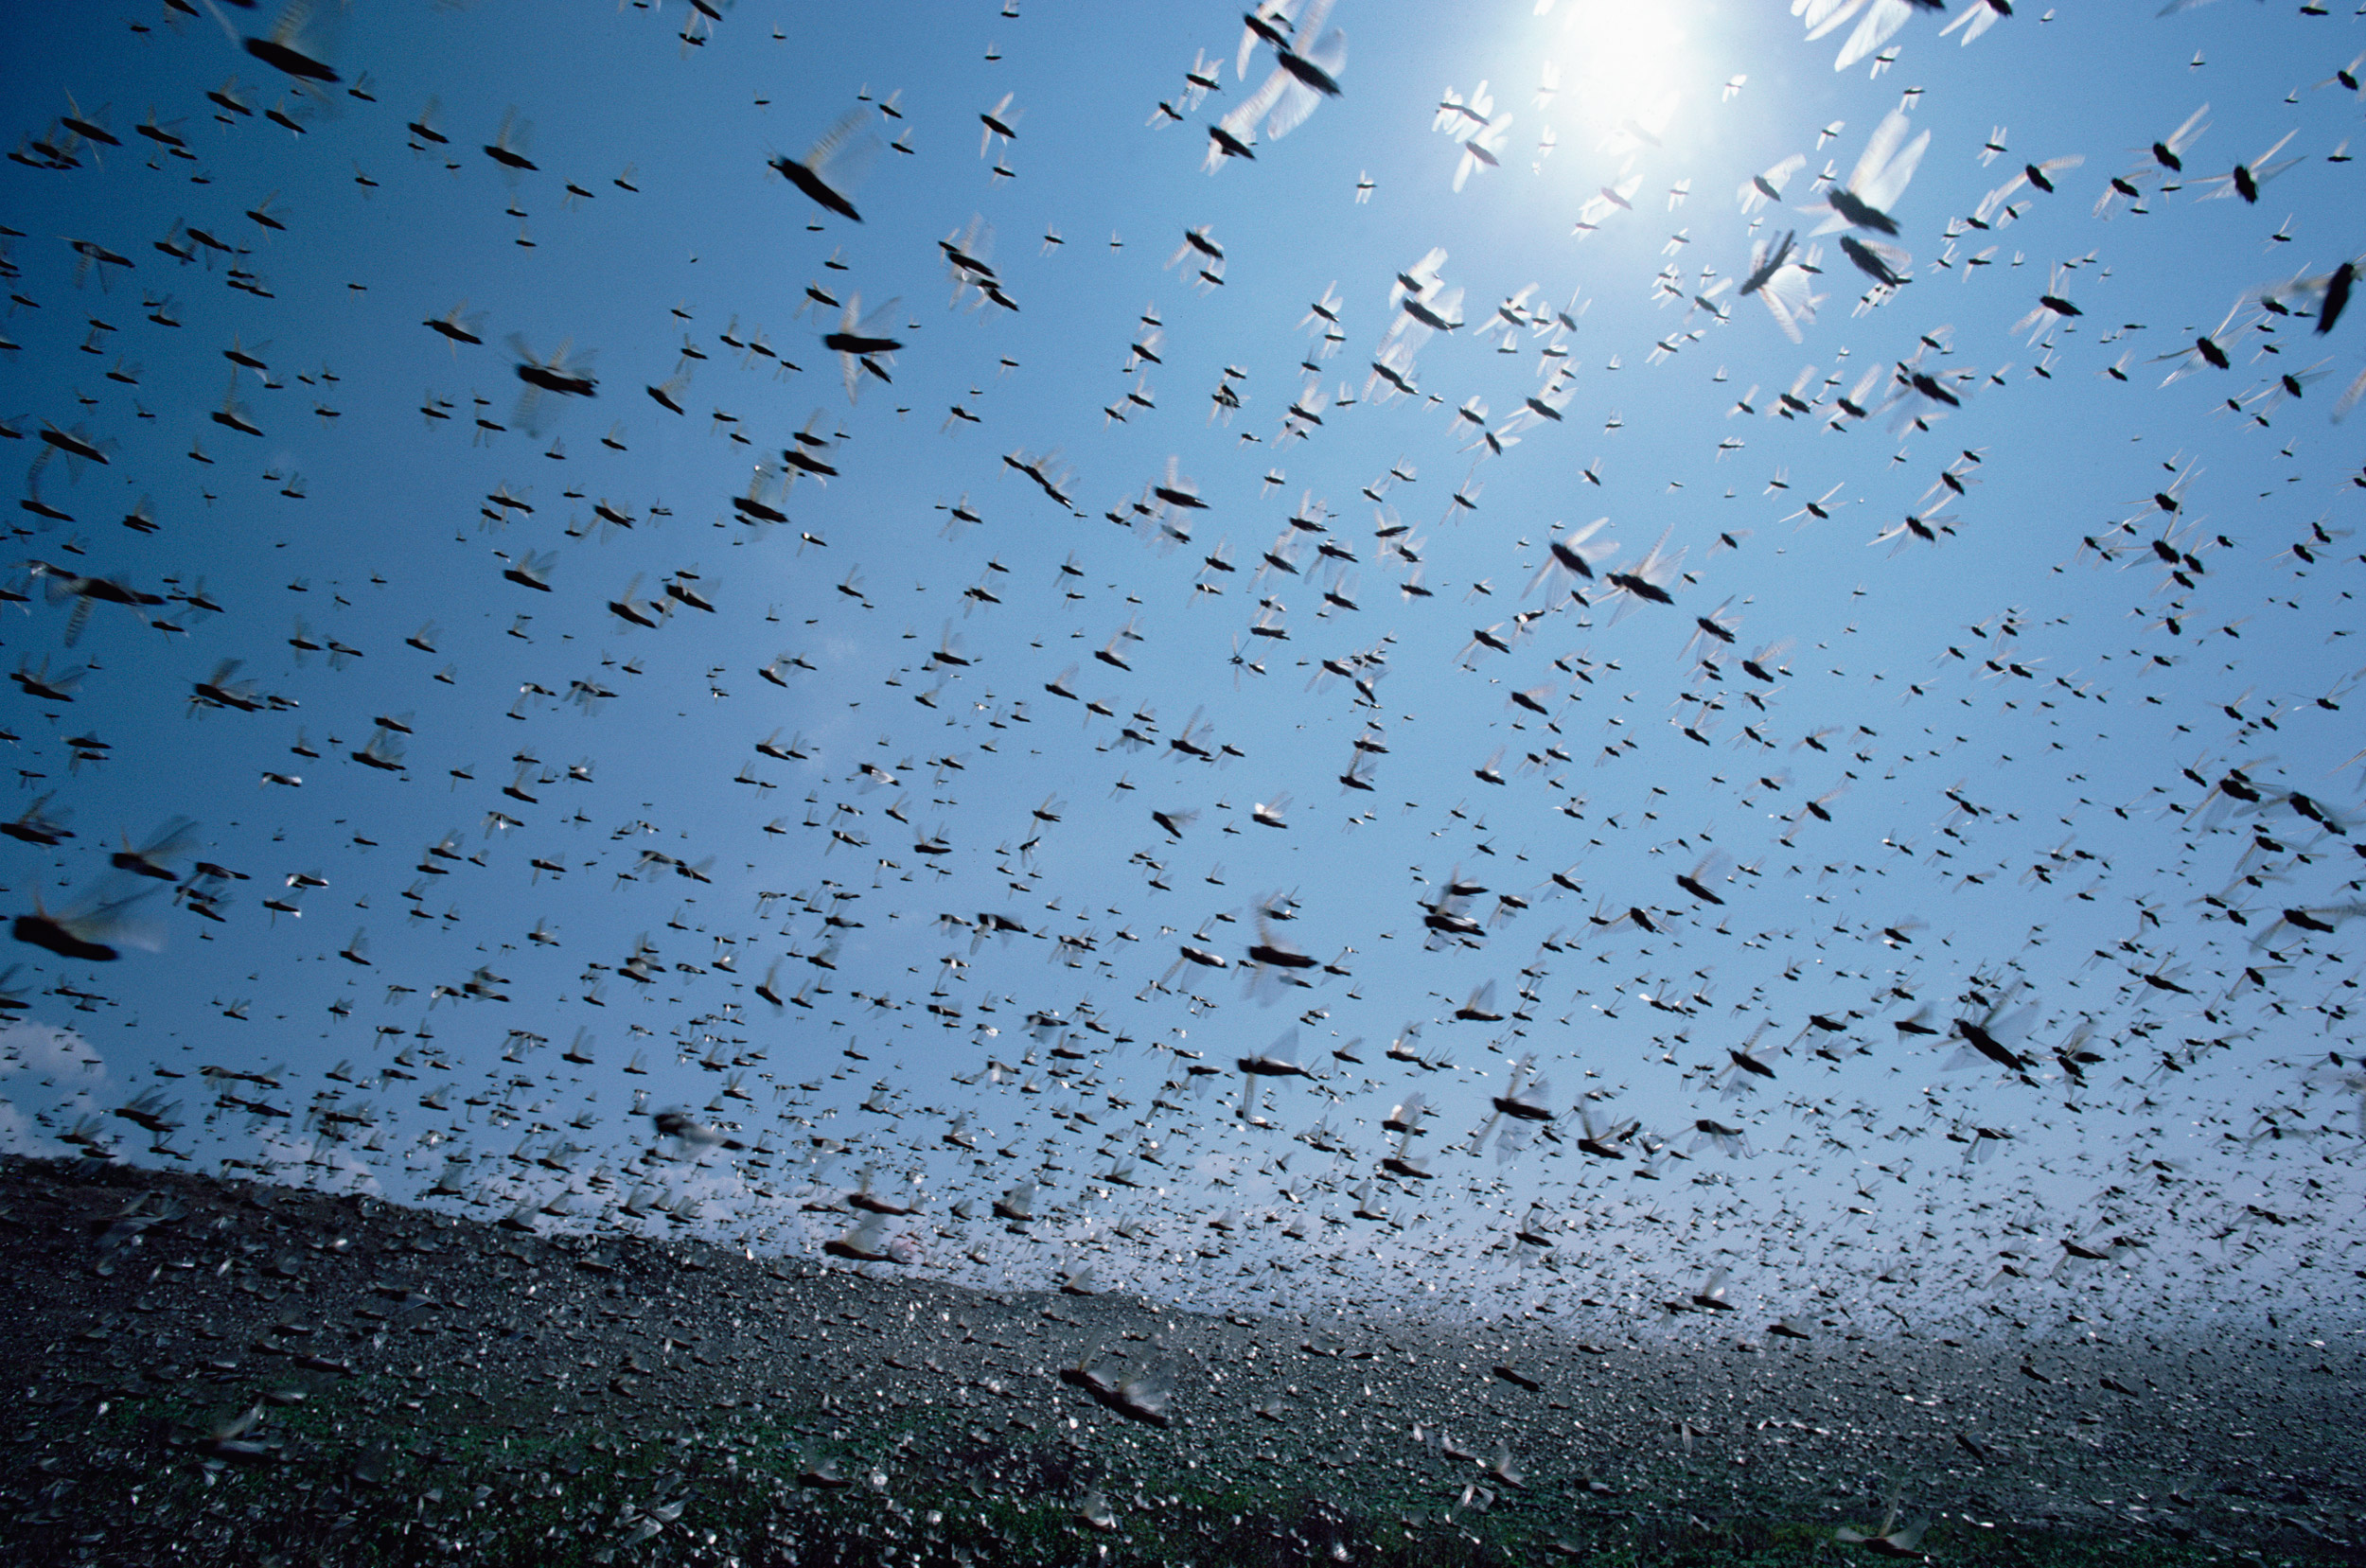
\includegraphics[height=6.7cm, center]{Invasion.jpg}\end{center}
}
\frame
{
  \frametitle{Konzept}
  \begin{itemize}
    \item Schwarmverhalten als Grundkonzept
    \item Prinzipiell keine festen Rollen sondern dynamische Handlungen
    \item Handlungen hängen prinzipiell von der aktuellen Position ab
    \item Grundlegende Funktion ist $f(x) = \frac 1 x$, wobei $x$ der Abstand zu einem anderen Objekt ist
  \end{itemize}
}

\subsection{Funktionen}
\frame{\frametitle{Algorithmus zur Auswahl der aktuellen Aktion}
\begin{itemize}
\item Funktionen, die Werte zwischen $0$ und $1$ zurückgeben.
\item Funktionen hängen vom Abstand des Nao zu anderen Entitäten ab
\item $0$ ist niedrigste Priorität und $1$ höchste
\item Alle Funktionen ausgewertet, die mit der höchsten Zahl wird ausgeführt
\end{itemize}
}
\frame
{
  \frametitle{Beispiele von Funktionen}
  \begin{itemize}
    \item \texttt{enemy\_owns\_ball}: Gibt zurück ob der der Gegner den Ball hat
    \item \texttt{run\_to\_ball}: Repräsentiert die Priorität zum Ball zu laufen
    \item \texttt{run\_to\_enemy\_goal}: Repräsentiert die Priorität zum gegnerischen Tor zu laufen. Das macht Sinn, wenn man den Ball hat
    \item \texttt{stay}: Einfach stehen bleiben. Das macht wenig Sinn und hat daher eine konstant niedrige Priorität
   \end{itemize}
}
\frame
{
  \frametitle{Beispielaufruf I}
  \begin{itemize}
    \item \texttt{run\_to\_ball}: 0.83    
    \item \texttt{run\_to\_own\_goal}: 0.451
    \item \texttt{run\_to\_enemy\_goal}: 0.034
    \item \texttt{stay}: 0.1
  \end{itemize}
}

\frame
{
  \frametitle{Beispielaufruf II}
  \begin{itemize}
    \item \colorbox{red}{\texttt{run\_to\_ball}: 0.83} \textcolor{red}{$\leadsto$} wird ausgewählt, da der Wert am höchsten ist 
    \item \texttt{run\_to\_own\_goal}: 0.451
    \item \texttt{run\_to\_enemy\_goal}: 0.034
    \item \texttt{stay}: 0.1
  \end{itemize}
}